\documentclass{article}
\author{}

\usepackage{graphicx}
\usepackage{wrapfig}
\usepackage{enumerate}
\usepackage{hyperref}
\usepackage{float}
\usepackage[margin = 2.25cm]{geometry}
\usepackage[table]{xcolor}
\usepackage{fancyhdr}
\hypersetup{
  colorlinks = true,
  urlcolor = blue
}
\setlength\parindent{0pt}
\pagestyle{fancy}
\fancyhf{}
\rhead{College of Engineering, Construction and Living Sciences\\Bachelor of Information Technology}
\lfoot{Practical 18 React 3: State \& Lifecycle Methods \\Version 1, 2020}
\rfoot{\thepage}

\begin{document}

\begin{figure}
	\centering
	
\includegraphics[width=50mm]{./img/logo.png}
\end{figure}

\title{College of Engineering, Construction and Living Sciences\\Bachelor of Information Technology\\IN608: Intermediate Application Development Concepts\\Level 6, Credits 15\\\textbf{Practical 18 React 3: State \& Lifecycle Methods}} 
\date{}
\maketitle

\textbf{Due Date:} 28/09/2020 at 5pm \\

In this practical, you will complete a series of tasks covering today's lecture. This practical is worth 1\% of the final mark for the IN608: Intermediate Application Development Concepts course. \\

Before you start, in your practicals repository, create a new branch called \textbf{18-practical}.

\section*{Task} 
Create a React app called \texttt{practical18state}. \texttt{cd} to \texttt{practical18state} \& install the following packages:
\begin{itemize}
  \item Axios - \texttt{npm i axios}
  \item He - \texttt{npm i he}
  \item Material Design for Bootstrap - \texttt{npm i mdbreact}
  \item React router - \texttt{npm i react-router-dom}
  \item React spinners - \texttt{npm i react-spinners}
\end{itemize}

Optionally, you can install all of them at once, i.e., \texttt{npm i axios he mdbreact react-router-dom react-spinners}. \\

Create a directory called \texttt{components}. Move \texttt{App.js} into \texttt{components}. Create two files called \texttt{OpenTDB.js} \& \texttt{Error.js}. In \texttt{OpenTDB.js}, create a function based component called \texttt{OpenTDB}. In \texttt{OpenTDB}, declare the following \texttt{state} variables:
\begin{verbatim}
  const [error, setError] = useState(null)
  const [isLoaded, setIsLoaded] = useState(false)
  const [data, setData] = useState([])
  const [url] = useState('https://opentdb.com/api.php?amount=5&type=boolean')
\end{verbatim}

Below the \texttt{state} variables, declare the following \texttt{useEffect}:
\begin{verbatim}
  useEffect(() => {
    const fetchData = async () => {
      await axios
        .get(url)
        .then((res) => {
          setIsLoaded(true)
          setData(res.data.results)
        })
        .catch((err) => {
          setIsLoaded(true)
          setError(err)
        })
    }
    fetchData()
  }, [url])
\end{verbatim}

In \texttt{Error.js}, create a function component which returns the message \texttt{404: Not Found.} in an \texttt{h1}.

\subsection*{What is happening?} 
You are using a promise based HTTP package called \texttt{axios} to request data from an API endpoint using the \texttt{GET} HTTP method. \texttt{then()} method is called \& returns a \texttt{Promise}. It takes up to two arguments: callback functions for the success and failure cases of the \texttt{Promise}. In our case, if success, set the state of \texttt{isLoaded} to \texttt{true} \& \texttt{data} to the response contents from the API request. If failure, set the state of \texttt{isLoaded} to \texttt{true} \& \texttt{error} to the error caught. \\

In \texttt{render()}, if there is an error display the \texttt{error} state's message in an \texttt{h1} element. If \texttt{isLoaded} is \texttt{false}, display a loading spinner using \texttt{react-spinners}. If \texttt{isLoaded} is \texttt{true}, return a \texttt{mdbreact} table containing the \texttt{data}. To use \texttt{mdbreact}, declare the appropriate \texttt{mdbreact} \& \texttt{bootstrap-css-only} imports. \\

You will notice some questions contain HTML entities. Encoding works slightly different in React \& you need to use \texttt{he} to do this. If there is no \texttt{data}, display the message \texttt{No data available.} in an \texttt{h1} element. \\

In \texttt{App.js}, call the \texttt{OpenTDB} \& \texttt{Error} components in the appropriate routes using \texttt{react-router-dom}. Your \texttt{App.js} file should look like the following:

\begin{verbatim}
  import React from 'react'
  import { Route, Switch } from 'react-router-dom'
  import Error from './Error'
  import OpenTDB from './OpenTDB'
  
  const App = () => {
    return (
      <div className='main-container'>
        <Switch>
          <Route path='/' component={OpenTDB} exact />
          <Route component={Error} />
        </Switch>
      </div>
    )
  }
  
  export default App  
\end{verbatim}

In \texttt{index.js} declare the following import:

\begin{verbatim}
  import { BrowserRouter } from 'react-router-dom'
\end{verbatim}

In \texttt{ReactDOM.render()}, wrap \texttt{BrowserRouter} around \texttt{App}. \\

\textbf{Note:} \texttt{className='main-container'} refers to the \texttt{index.css} style used in the code examples.

\subsection*{Expected Output} 
Run the command \texttt{npm start} then navigate to \href{http://localhost:3000/}{http://localhost:3000/} \\

\begin{figure}[H]
  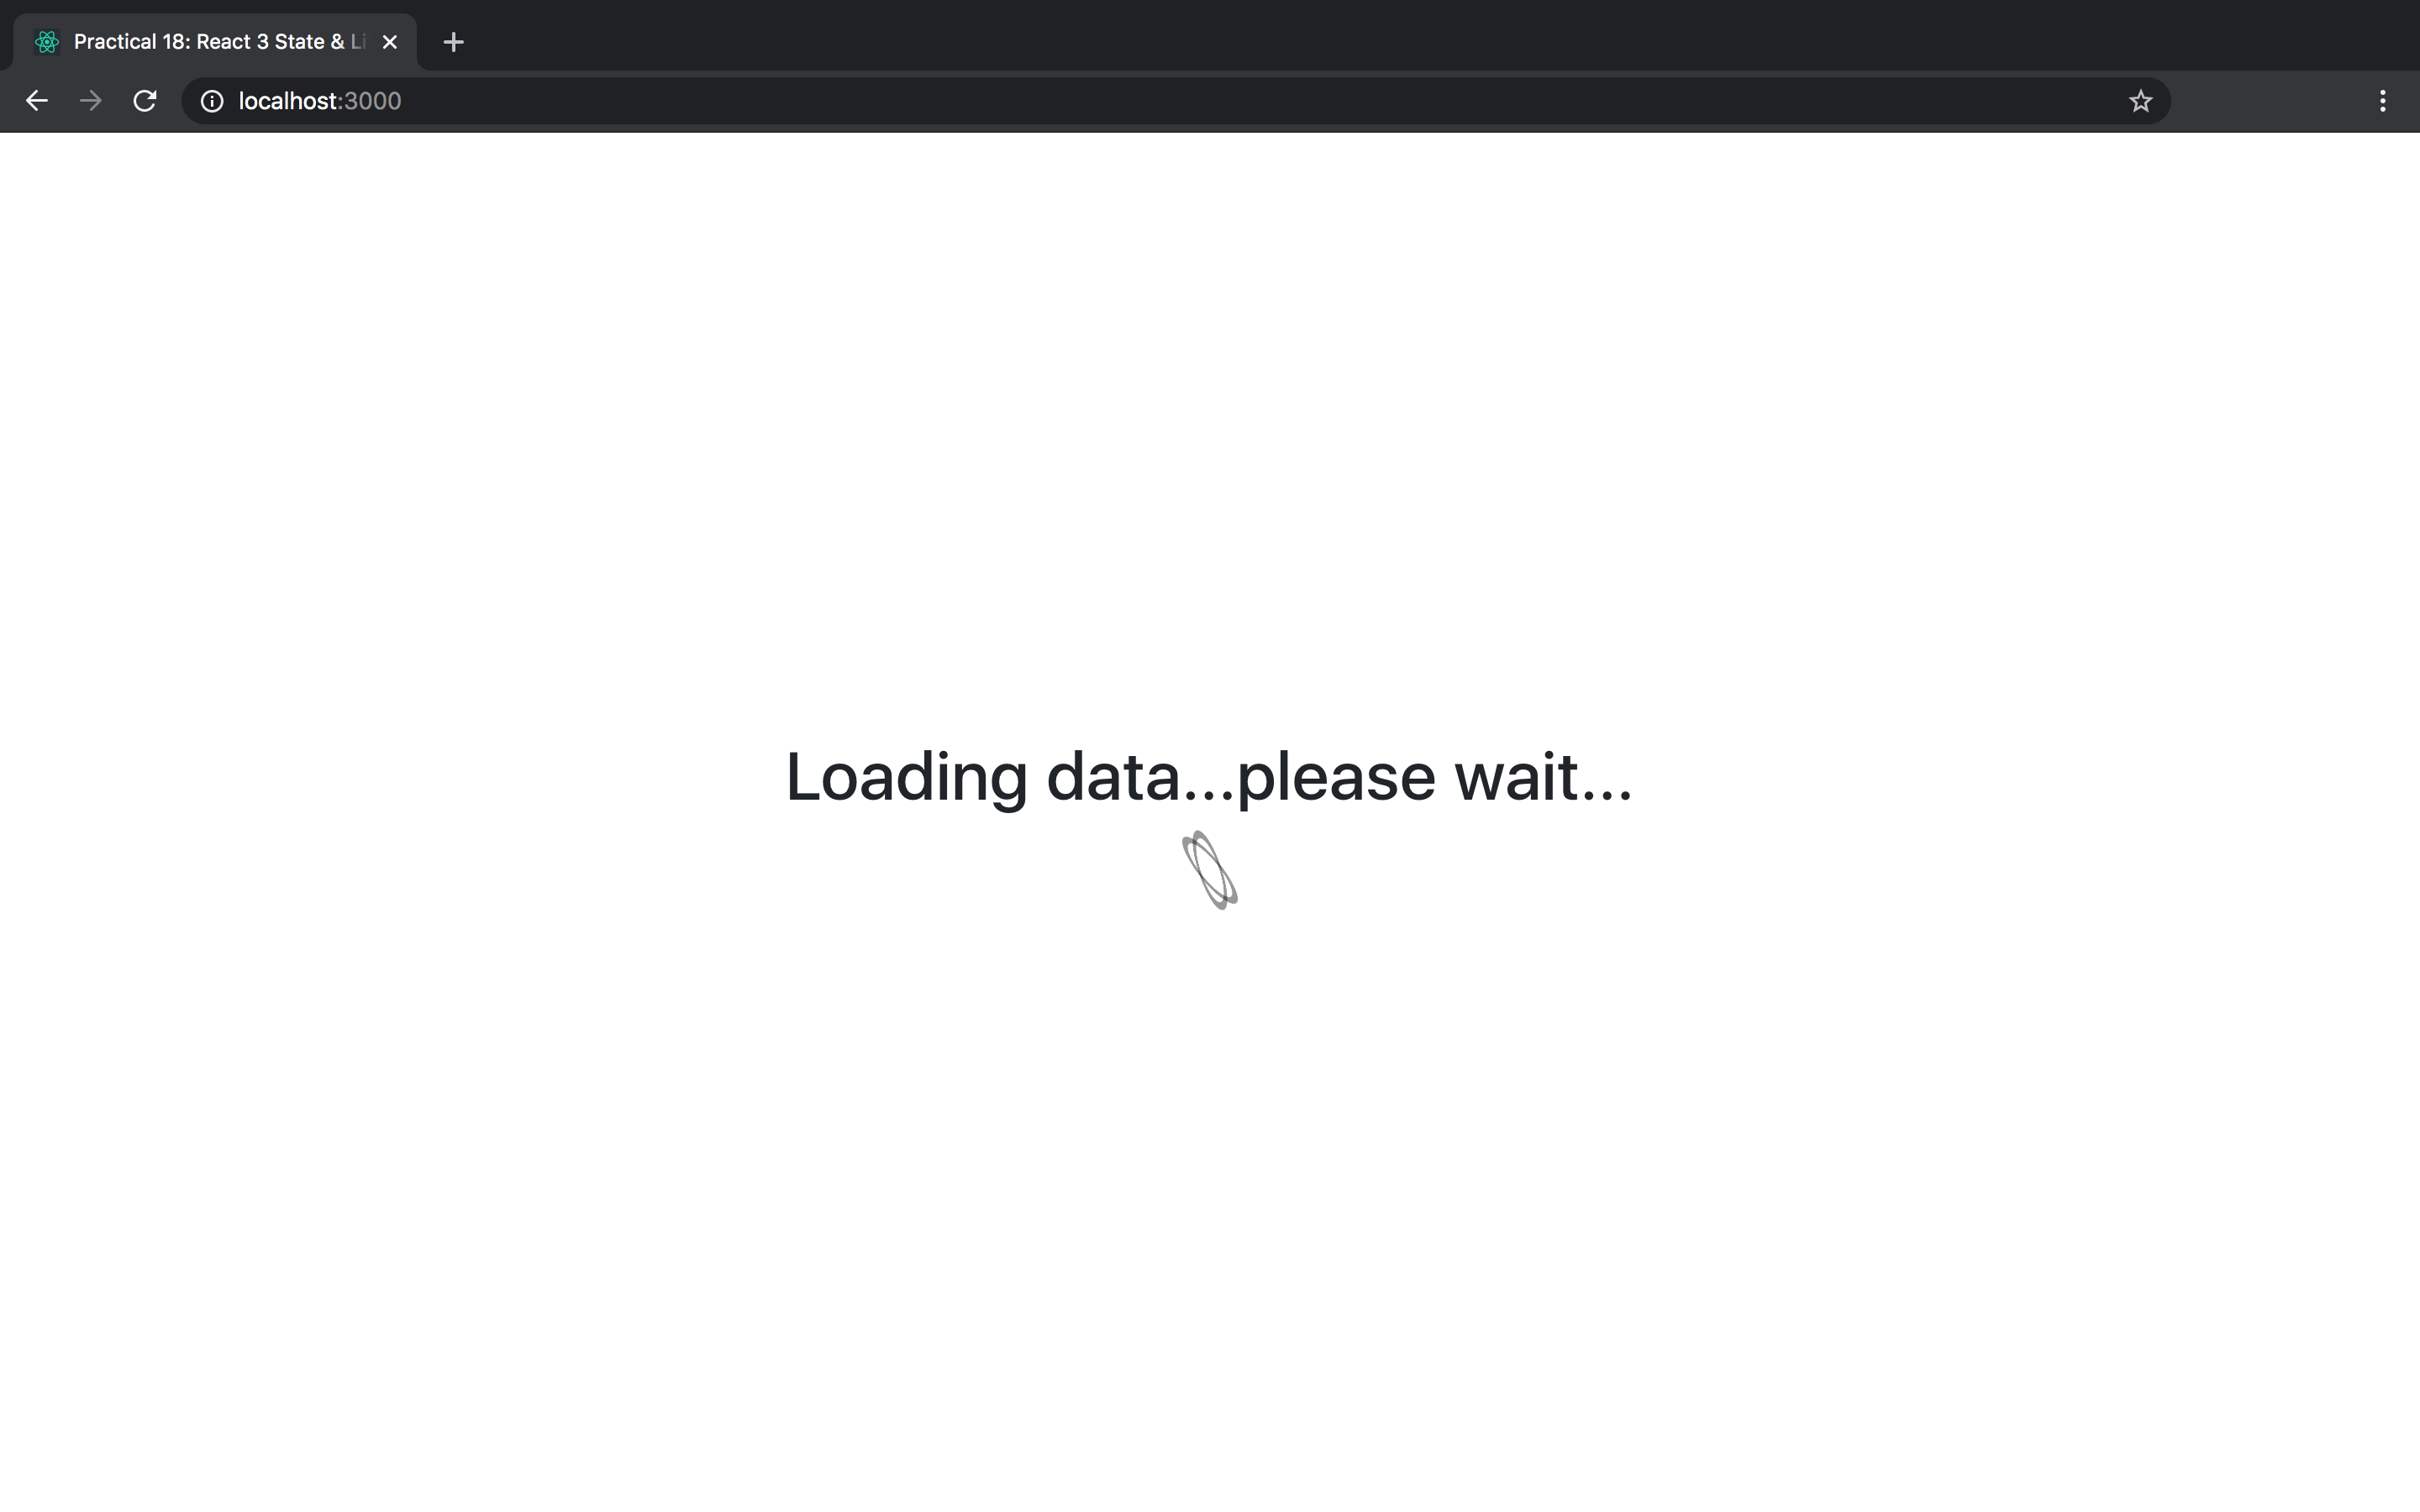
\includegraphics[width=175mm, height=105mm]{./img/18-expected-opentdb-1.png}
  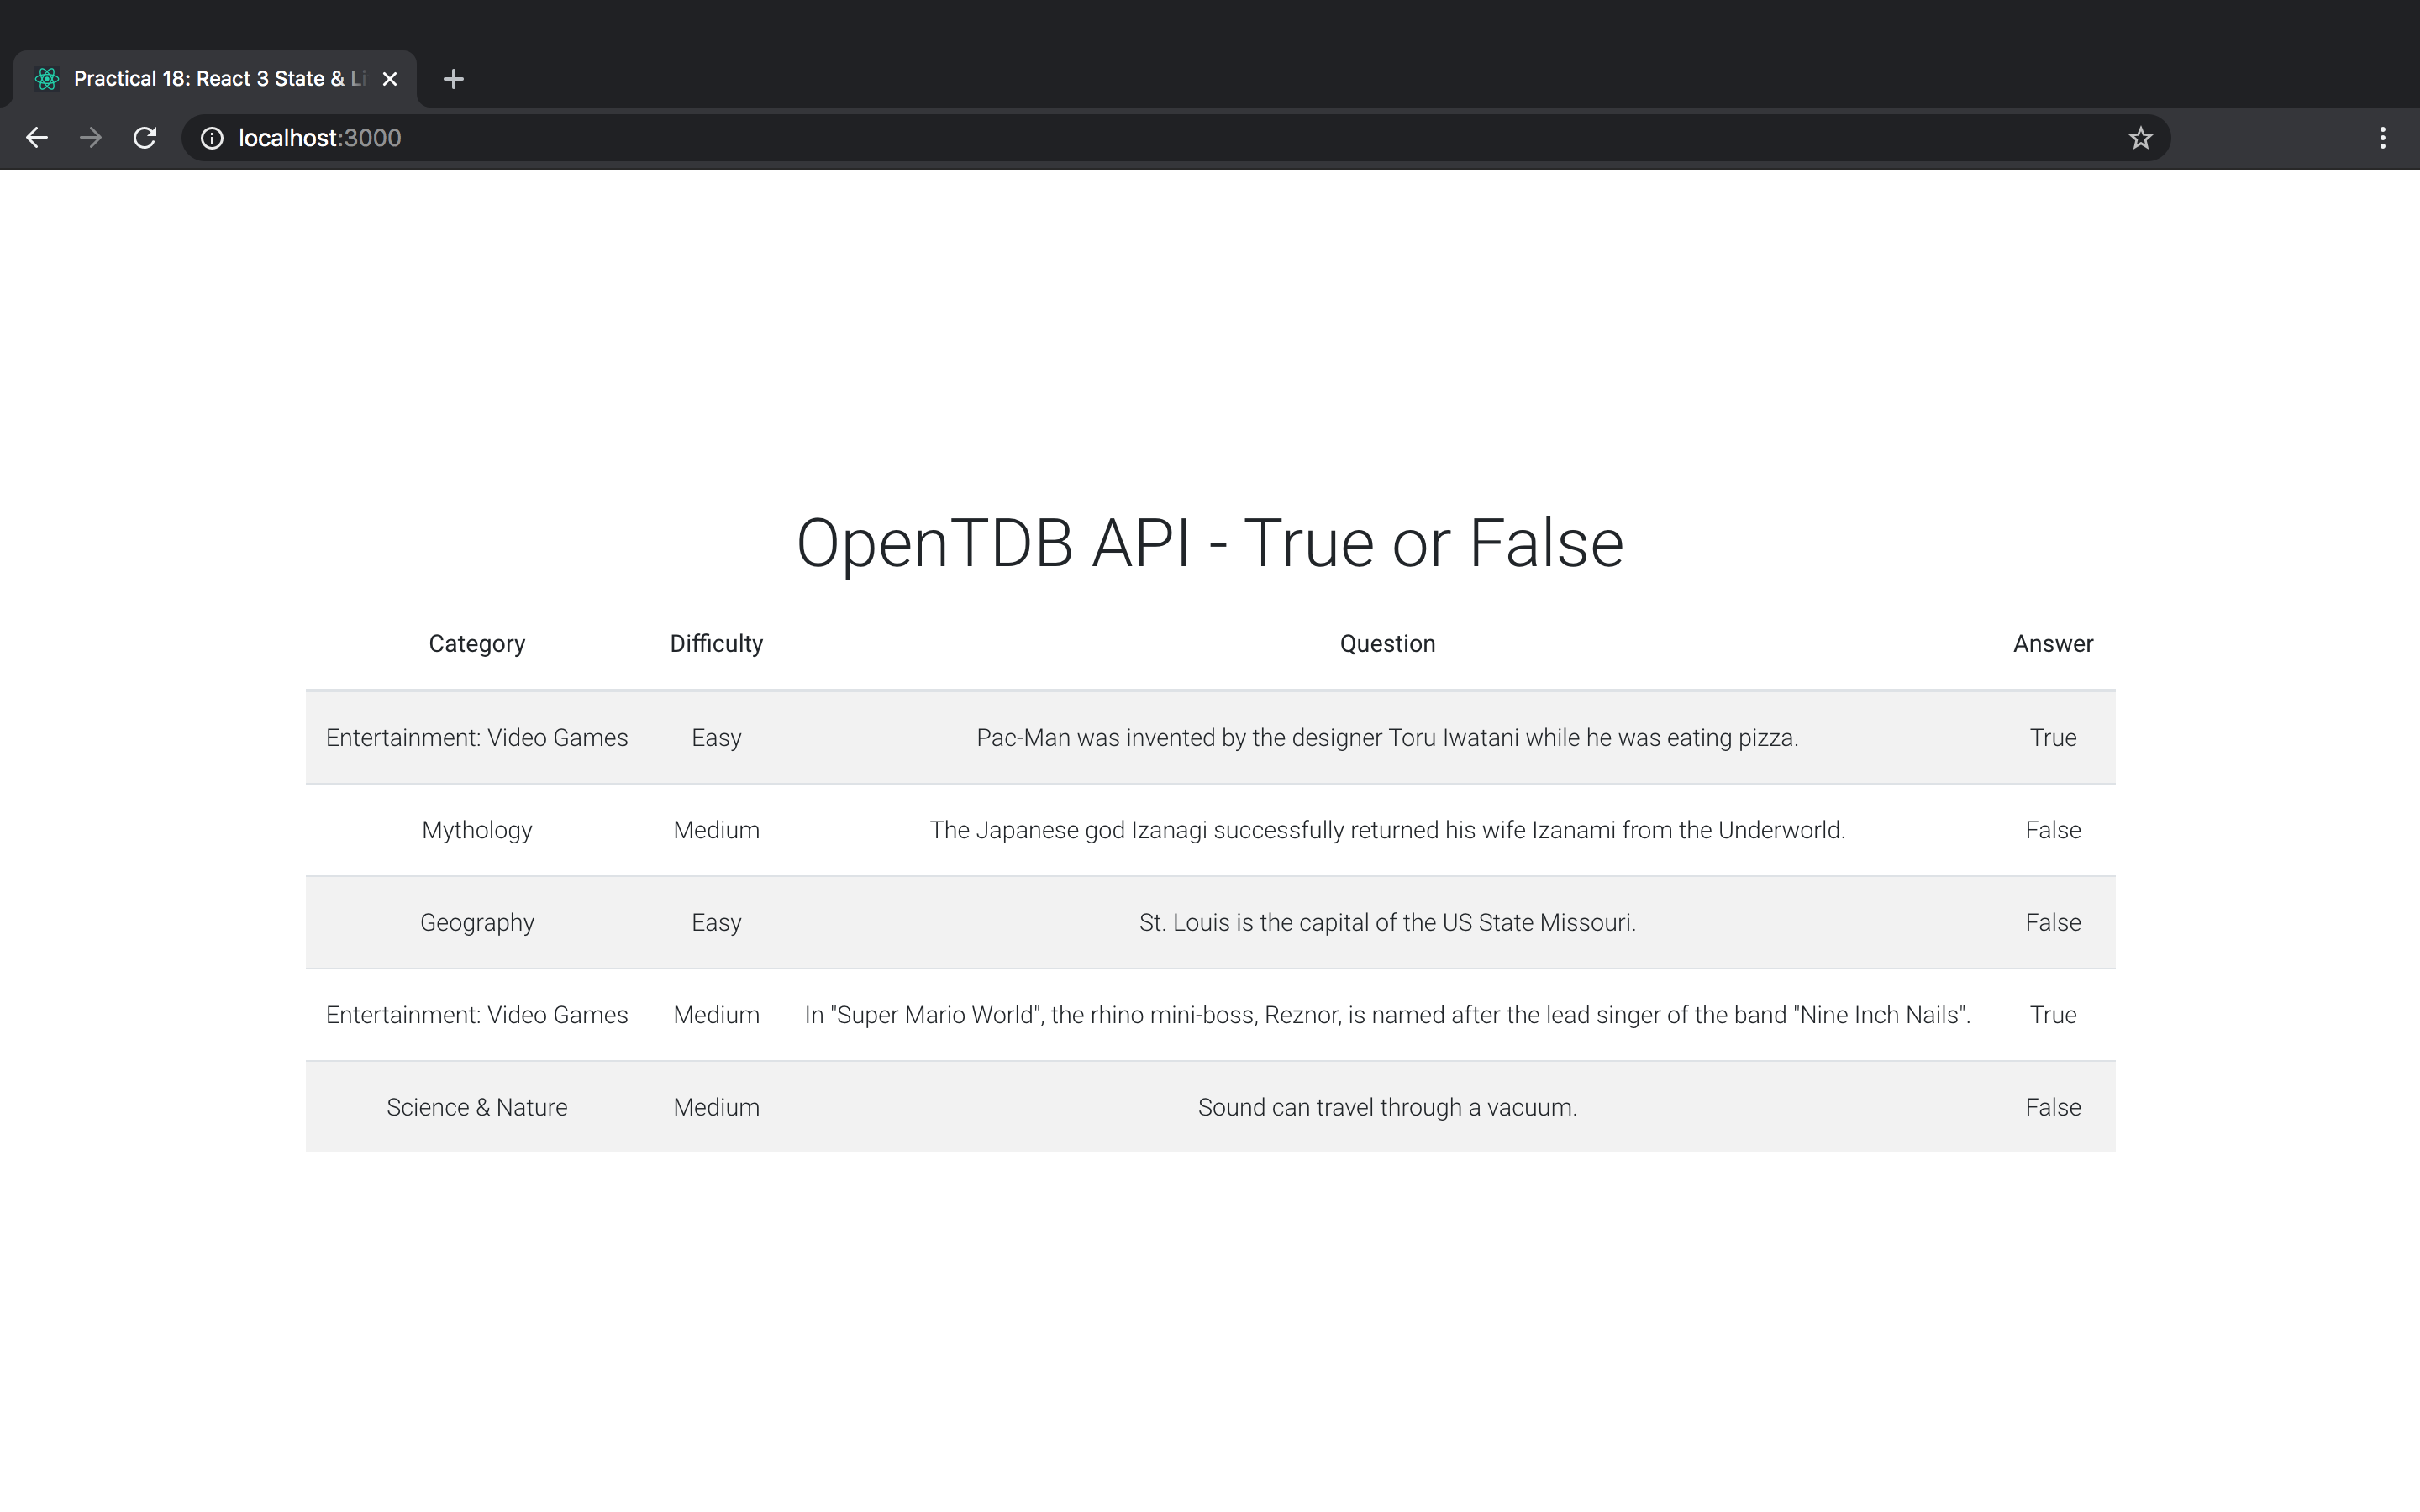
\includegraphics[width=175mm, height=105mm]{./img/18-expected-opentdb-2.png}
\end{figure}

\begin{figure}[H]
  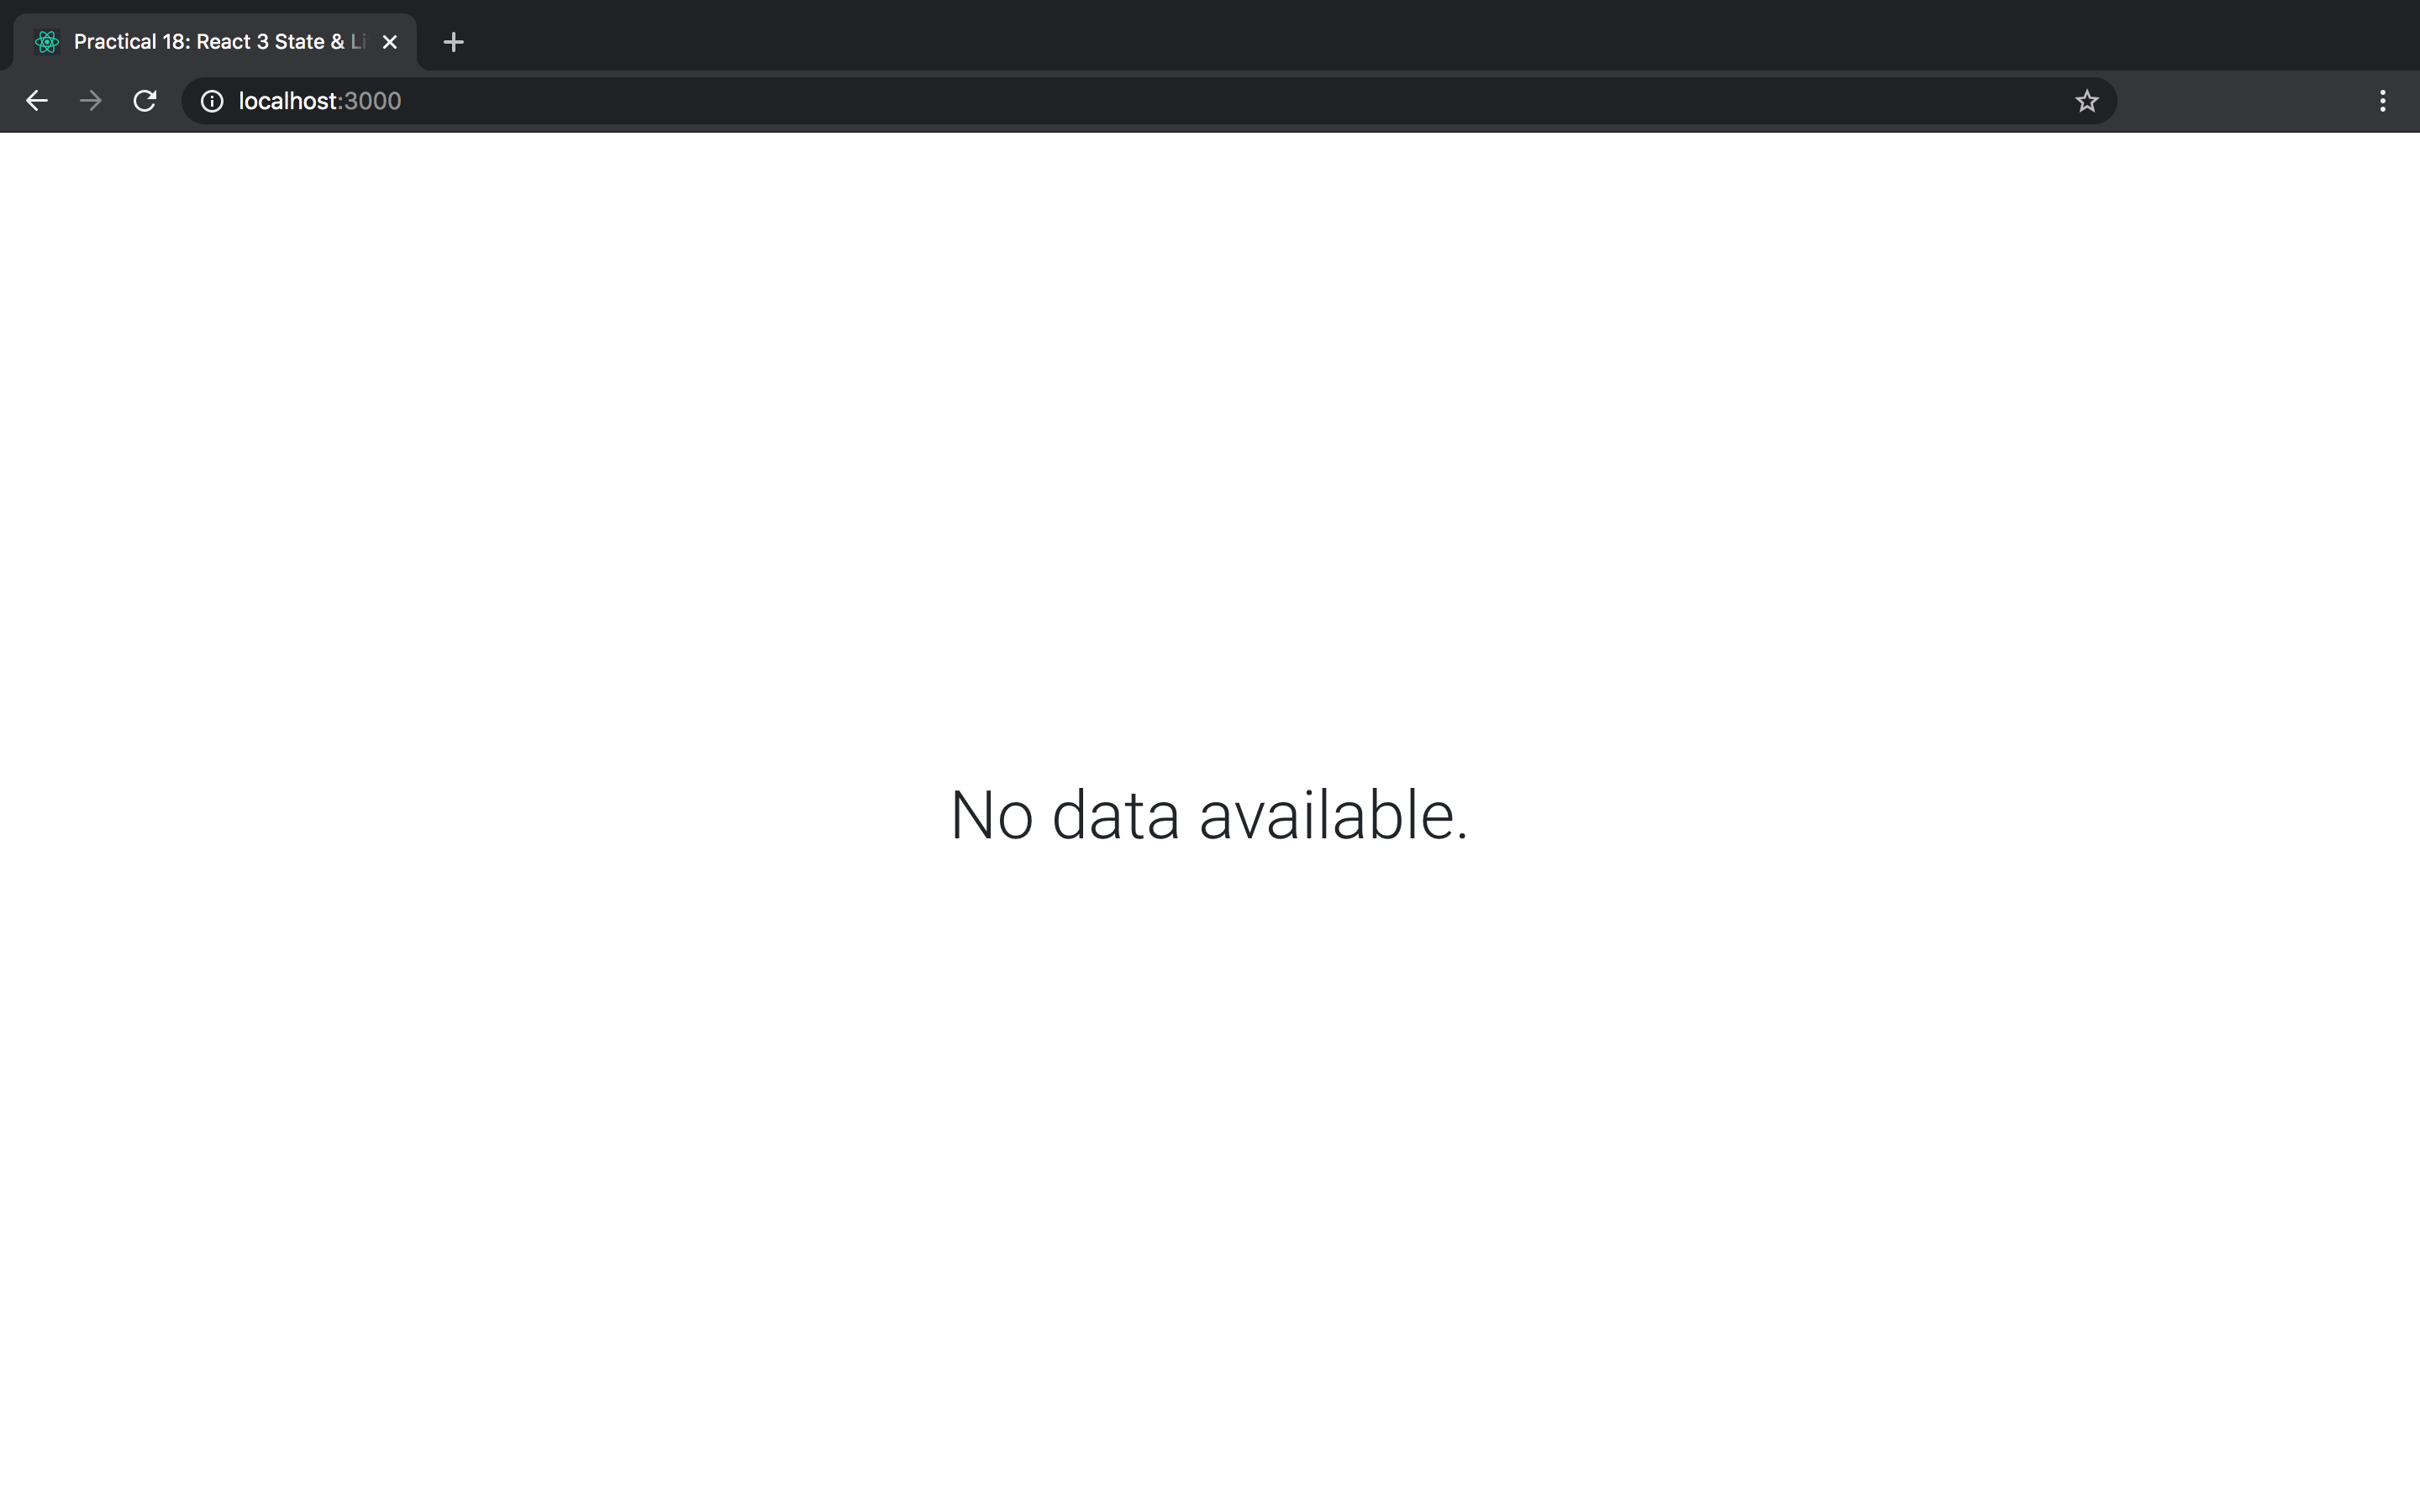
\includegraphics[width=175mm, height=105mm]{./img/18-expected-opentdb-3.png}
  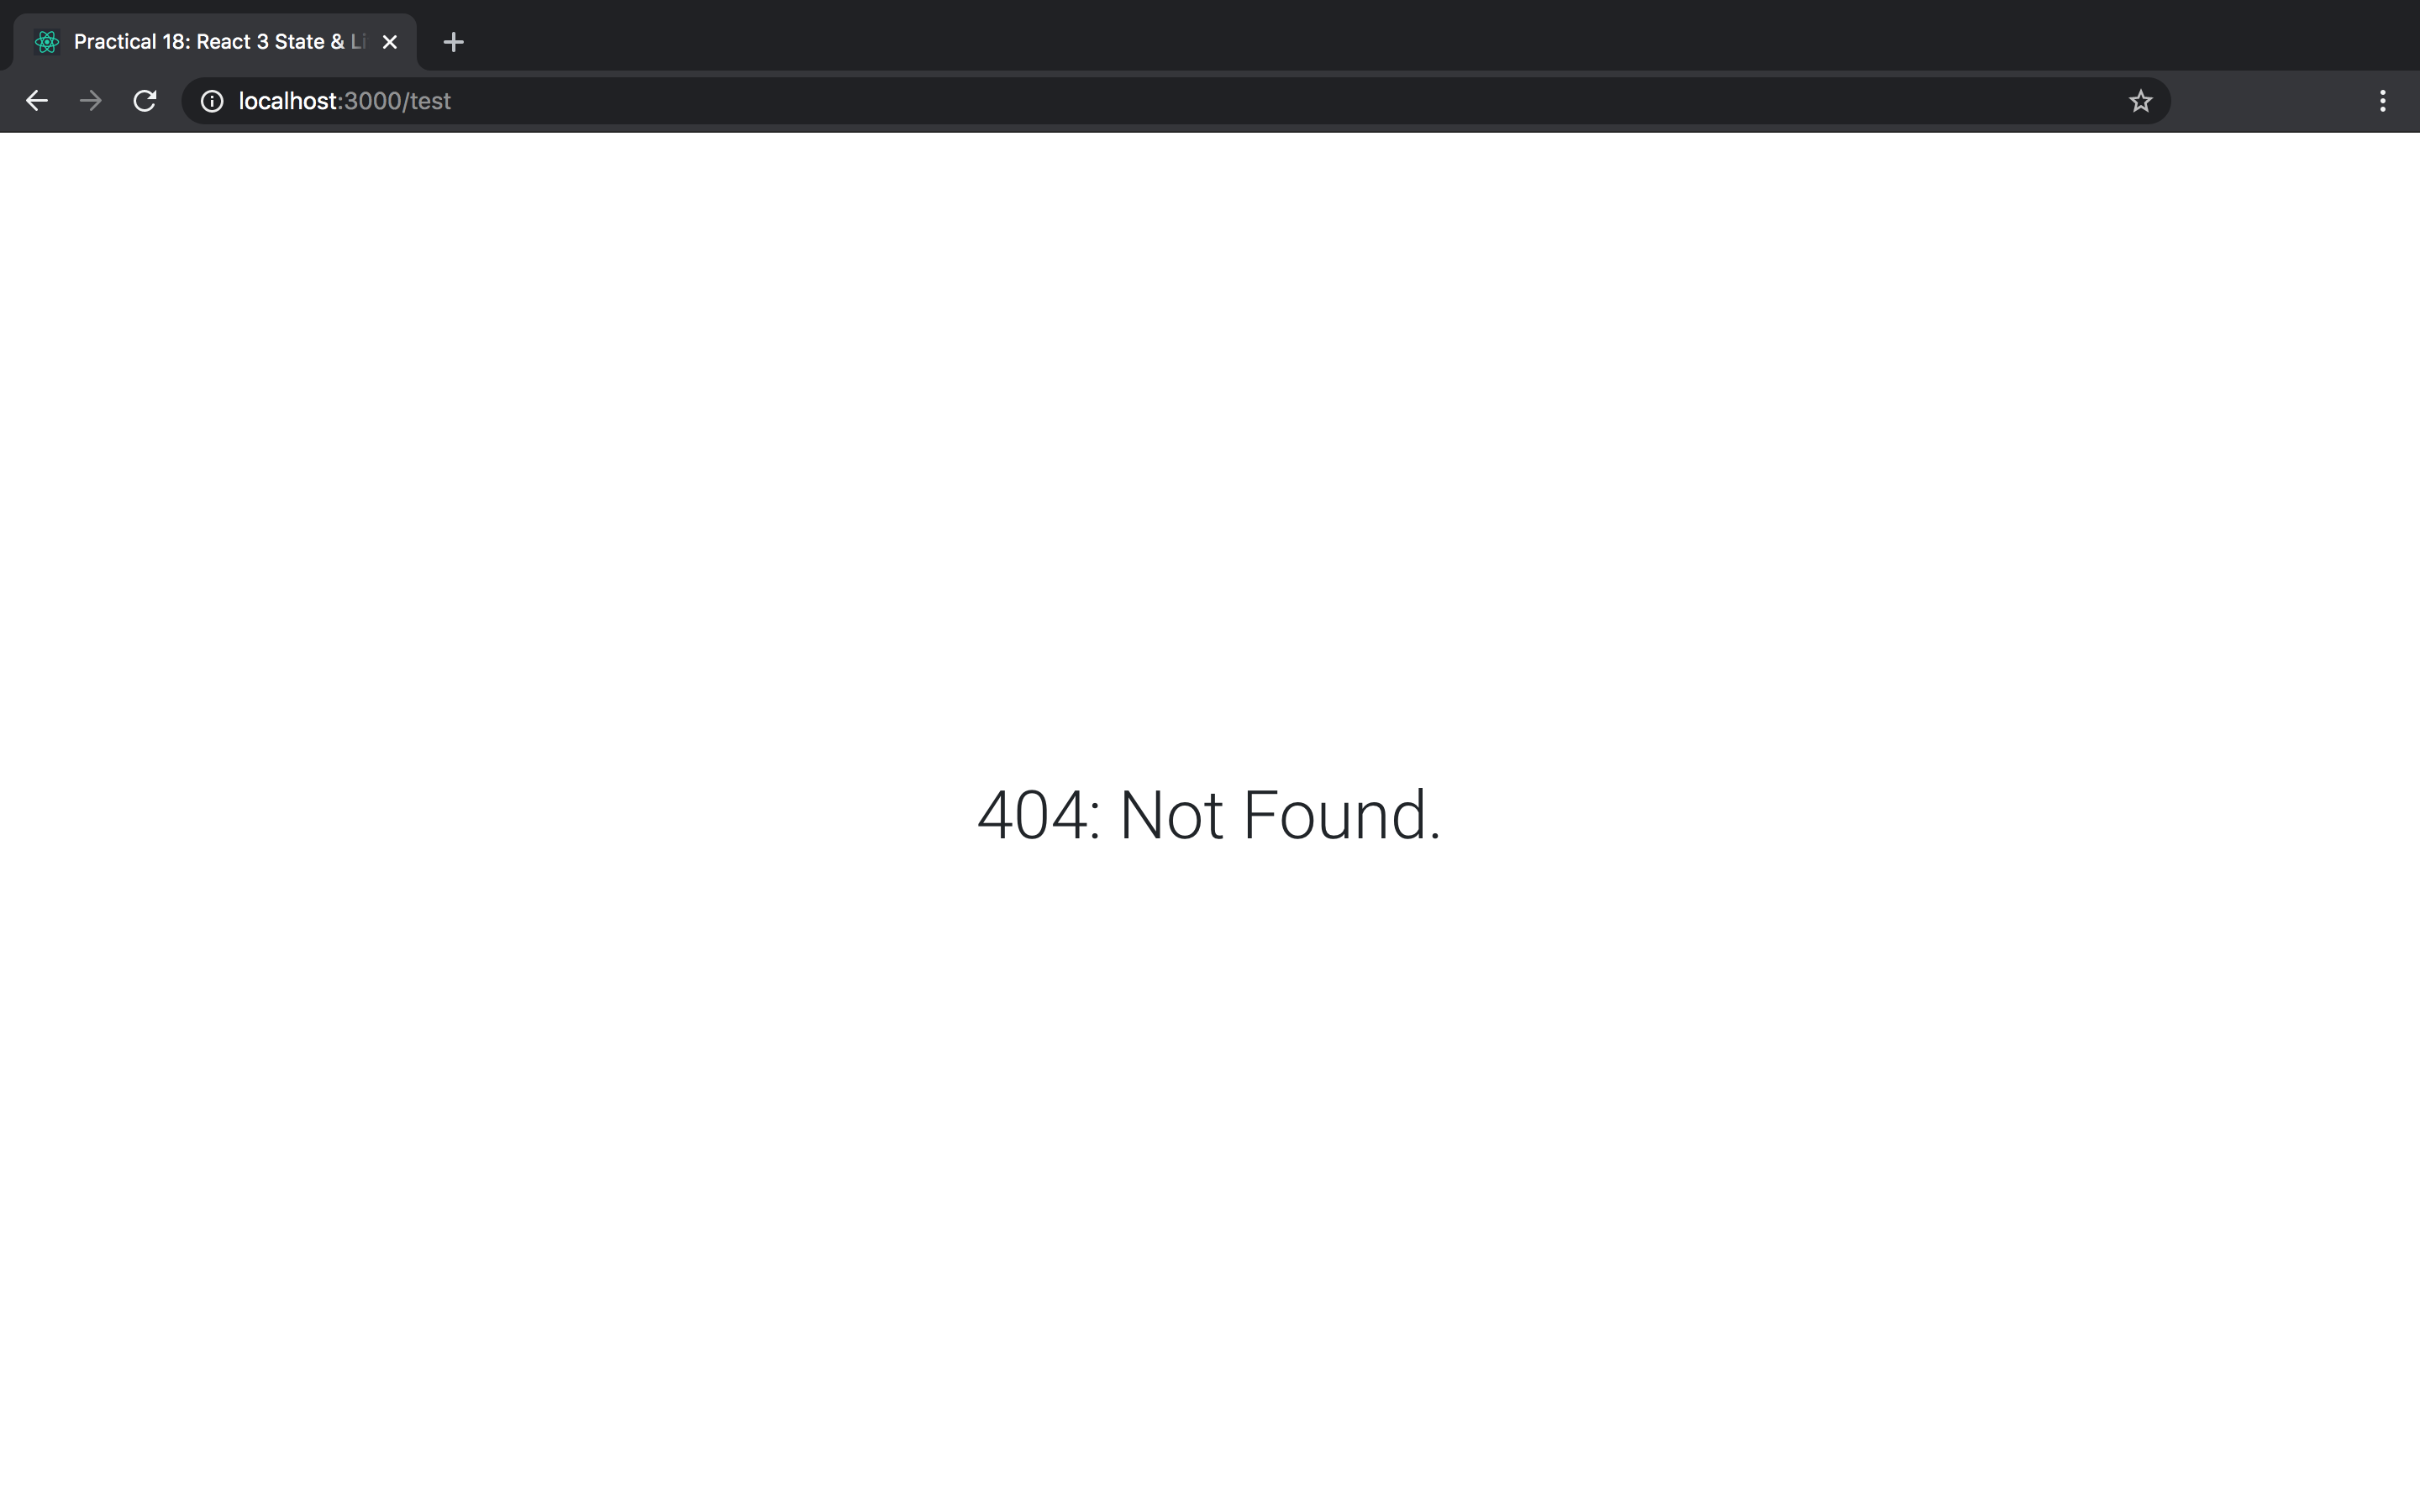
\includegraphics[width=175mm, height=105mm]{./img/18-expected-opentdb-4.png}
\end{figure}

\begin{figure}[H]
  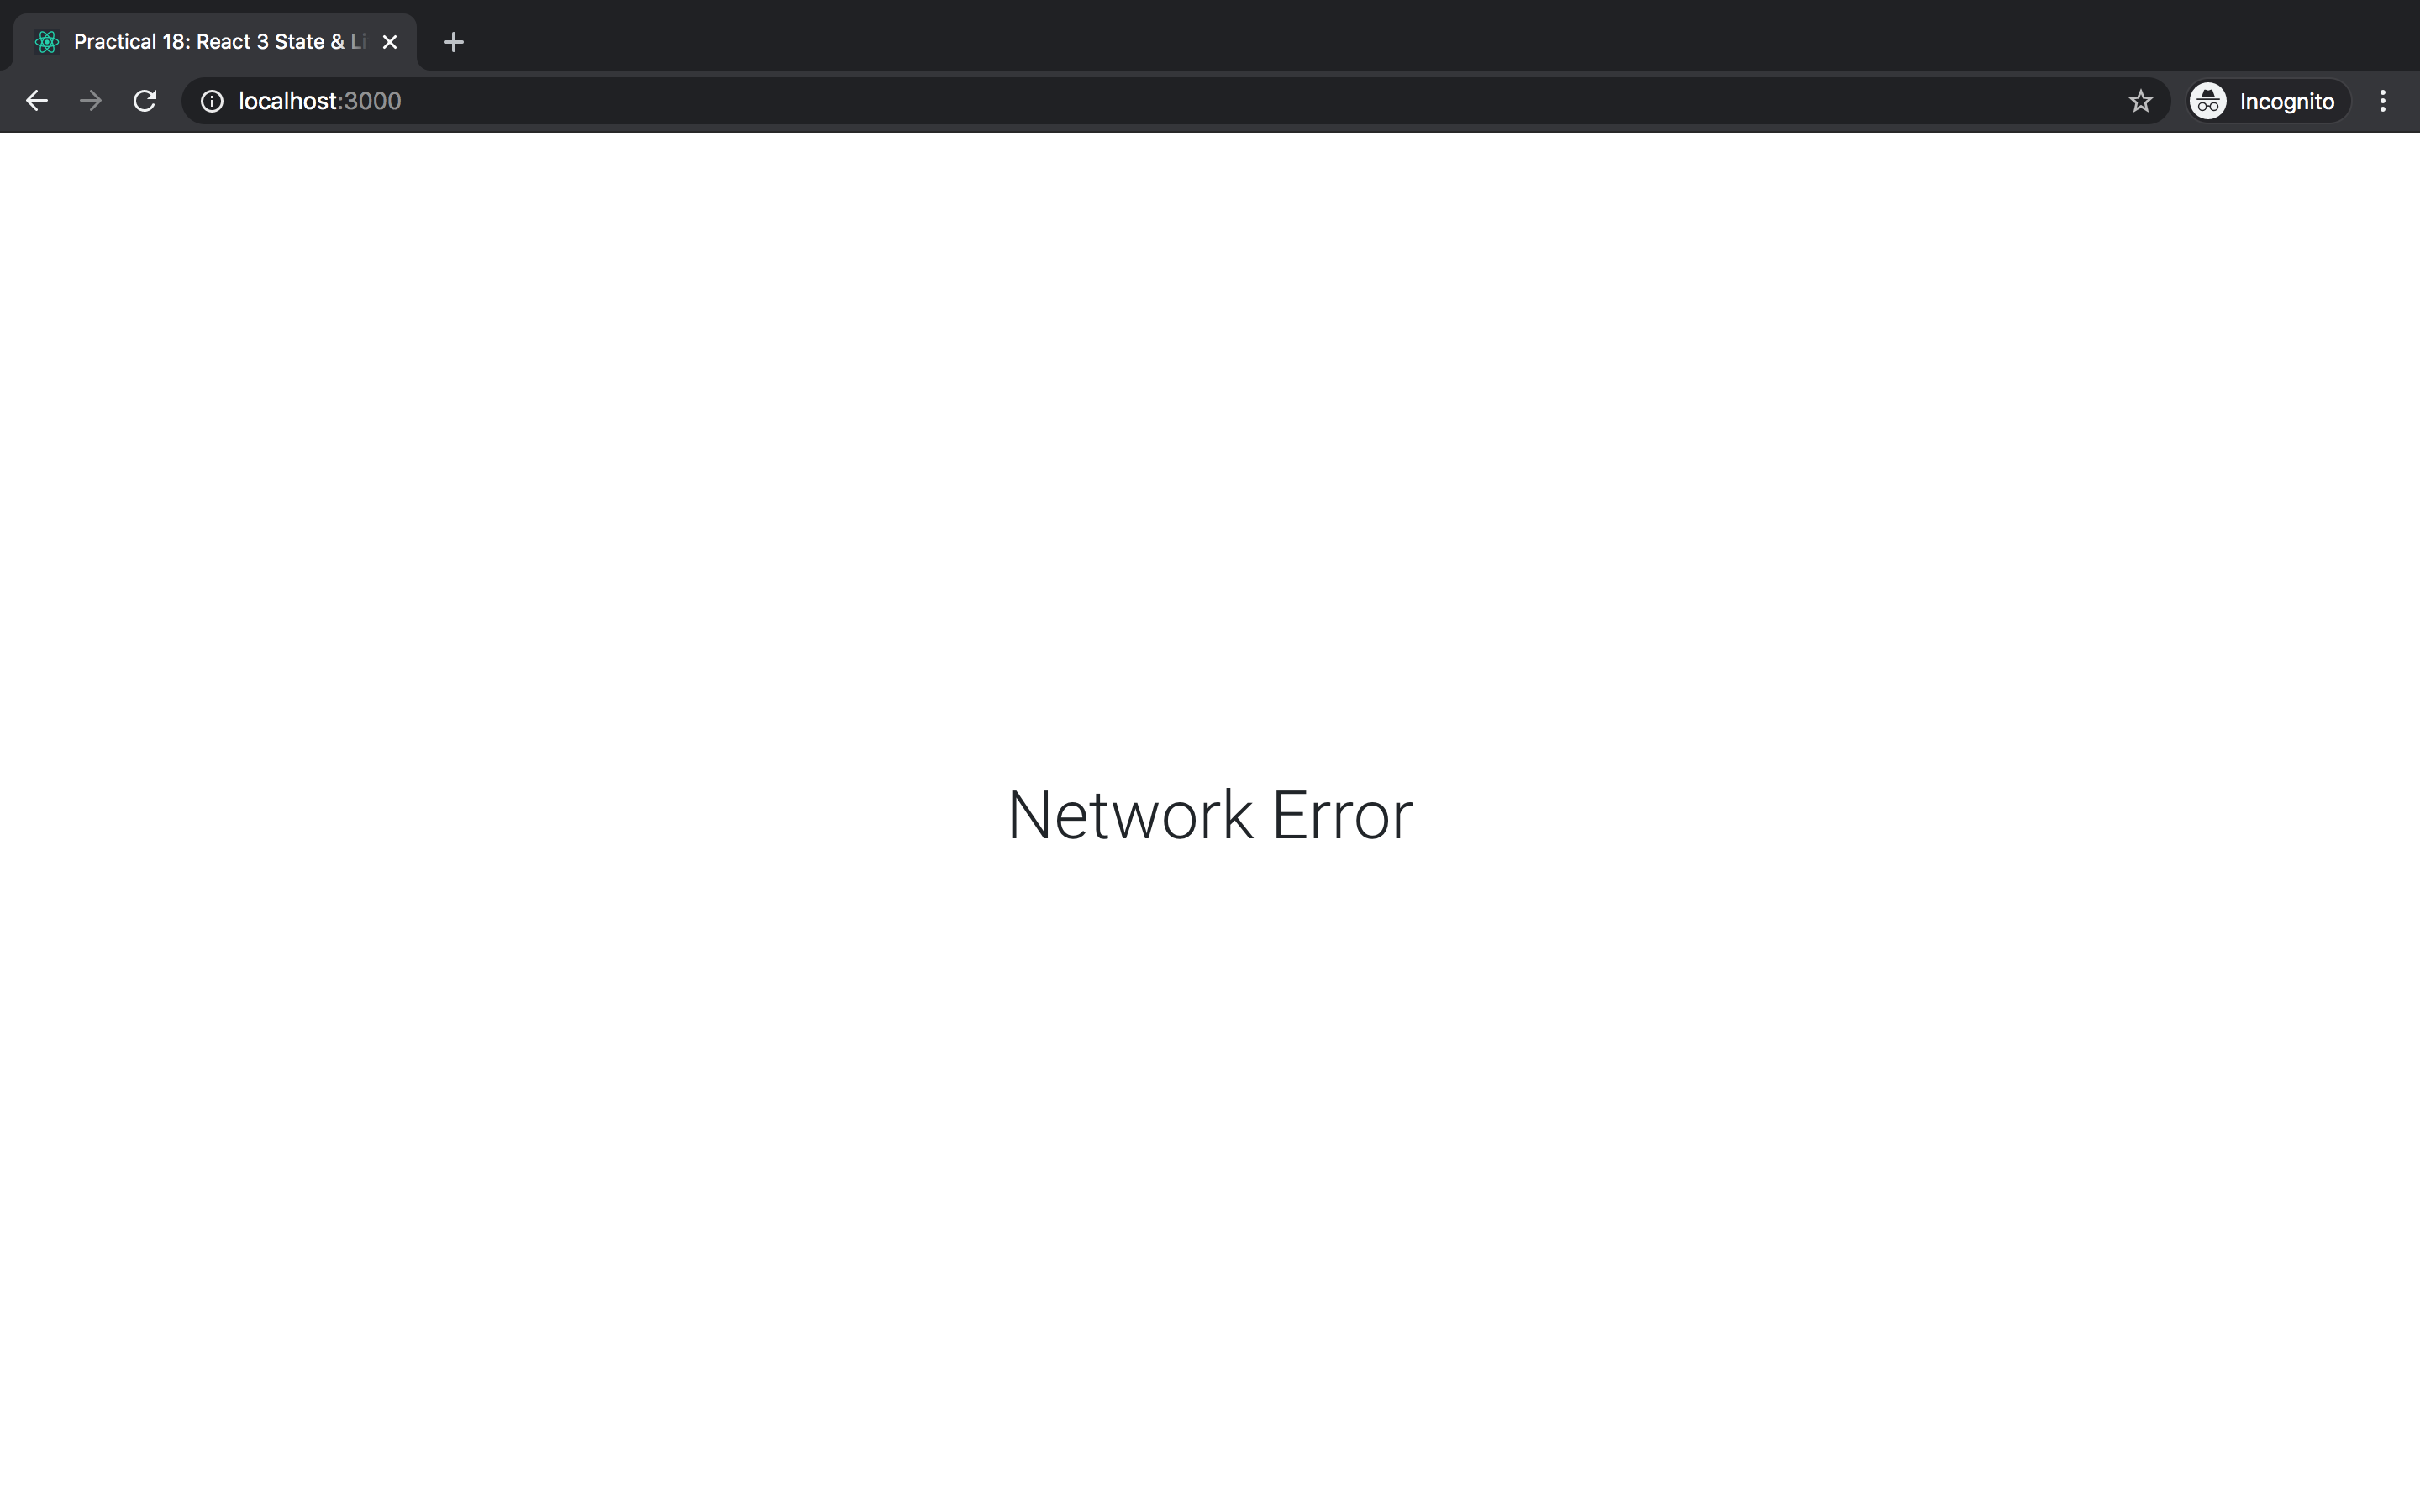
\includegraphics[width=175mm, height=105mm]{./img/18-expected-opentdb-5.png}
\end{figure}

\textbf{Deployment link:} \href{https://int-app-dev-practical-18.herokuapp.com/}{https://int-app-dev-practical-18.herokuapp.com/} 

\subsection*{Resources} 
\begin{itemize}
  \item \href{https://opentdb.com/}{OpenTDB API}
  \item \href{https://www.npmjs.com/package/axios/}{Axios}
  \item \href{https://www.npmjs.com/package/he/}{He}
  \item \href{https://mdbootstrap.com/}{Material Design for Bootstrap}
  \item \href{https://www.npmjs.com/package/mdbreact/}{Material Design for Bootstrap - npm}
  \item \href{https://www.npmjs.com/package/react-spinners/}{React spinners}
  \item \href{https://reactrouter.com}{React router}
  \item \href{https://www.npmjs.com/package/react-router/}{React router - npm}
\end{itemize}
 
\end{document}